\begin{frame} \frametitle{Motivation}
\begin{block} {Underwater?}
\begin{columns}
\column{.43\textwidth}
\centering
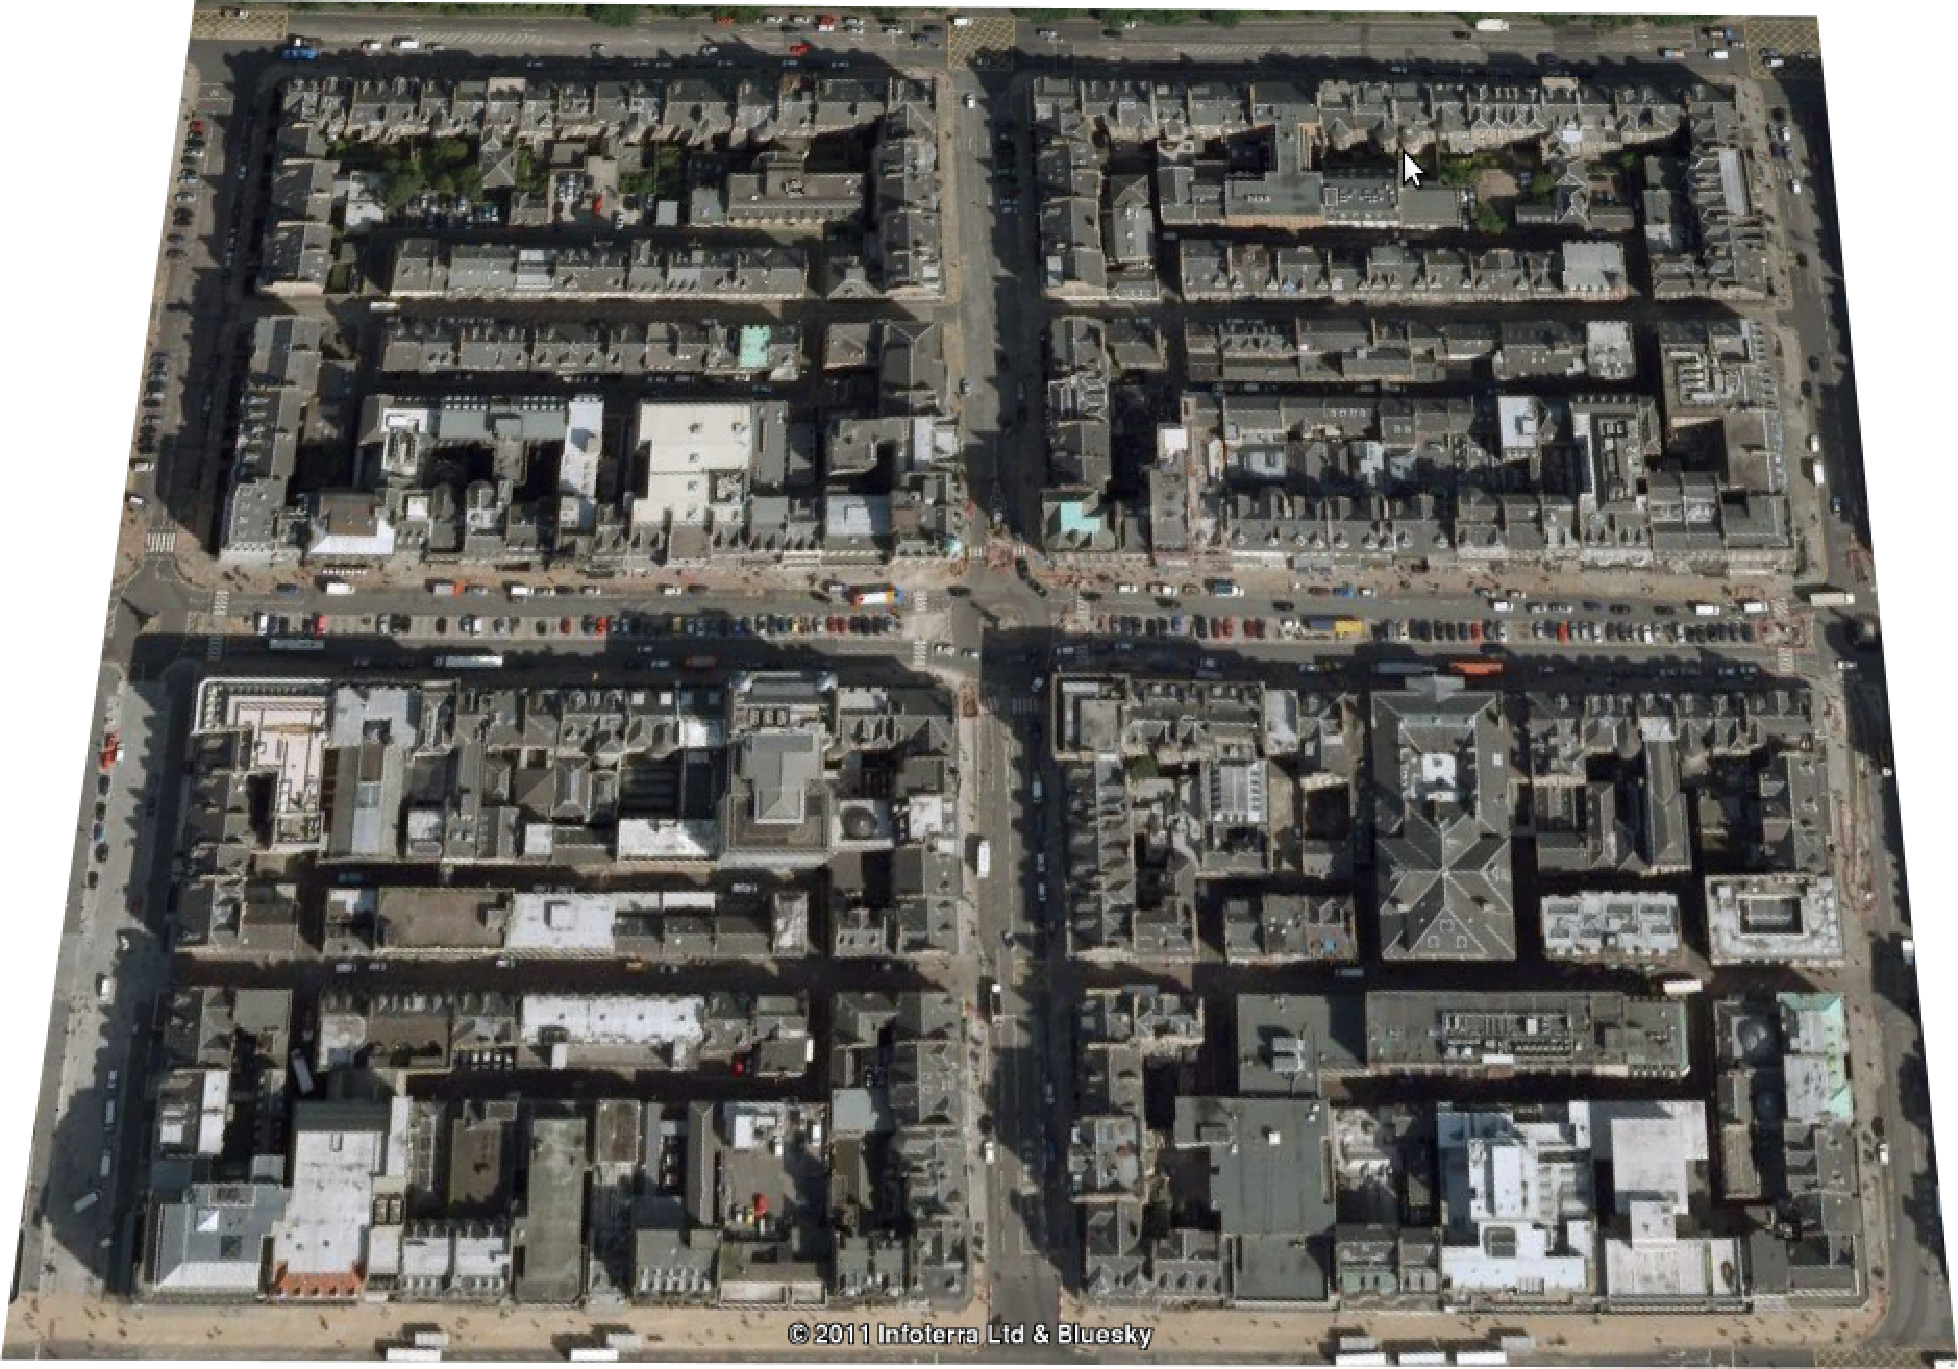
\includegraphics[width=0.8\linewidth]{fig/edinburgh.pdf} \\
Edinburgh, city centre. \\ 
$ 55^{\circ}57 ^{\backprime}16 ^{\backprime \backprime}  N  3^{\circ} 11 ^{\backprime} 58 ^{\backprime \backprime}  W $ \\
Elevation: $66 m$ \\
Area: $\approx 400 \times 300 m $
%%%%%%%%%%%%%%%%%%%%%%%%%%%%%%%%%%%%%%%%
\column{.1\textwidth}
\textit{... 1300 km away ...}
%%%%%%%%%%%%%%%%%%%%%%%%%%%%%%%%%%%%%%%%
\column{.43\textwidth}
\centering
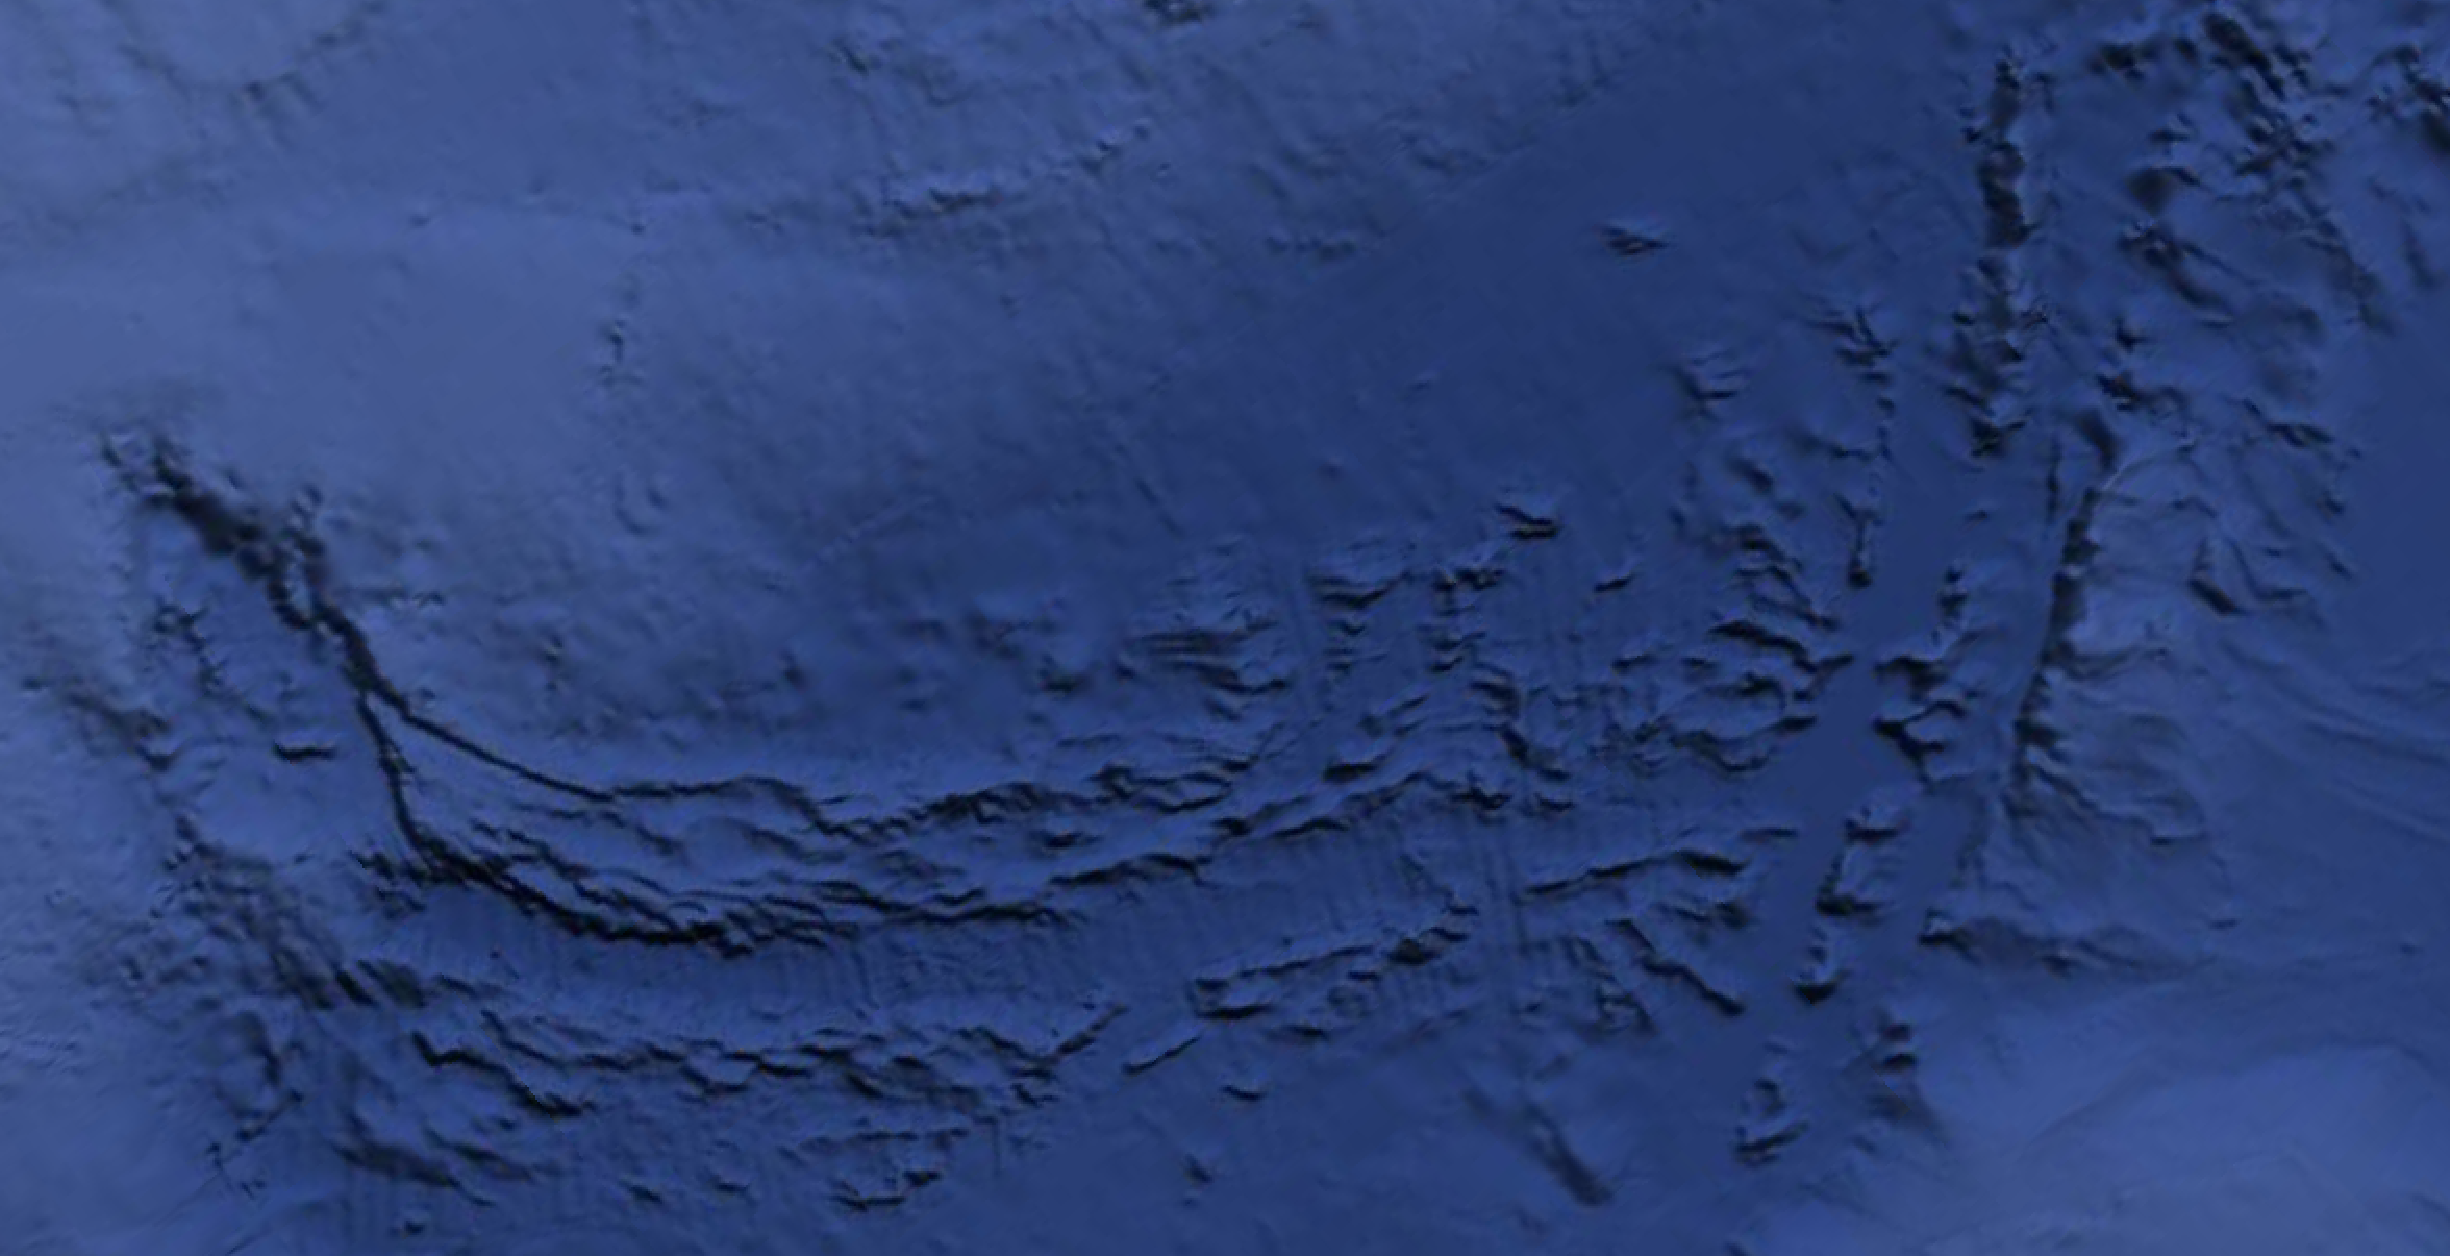
\includegraphics[width=0.8\linewidth]{fig/norwegianSea.pdf} \\
Norwegian sea. \\
$ 66^{\circ}  52 ^{\backprime} 46 ^{\backprime \backprime} N  3^{\circ}  36 ^{\backprime}  21 ^{\backprime \backprime} W $ \\
Elevation: $-3335 m$ \\
Area: $ \approx 700 \times 300 km $
\end{columns}
\end{block}

\begin{block} {Why navigation?}
	To be able to navigate the robot within the environment - we need to know it's position - to \textbf{localise} it.
\end{block}
%%mention applications: exploration, special tasks, mapping, inspections, military
\end{frame}